\documentclass[journal]{IEEEtran}


\usepackage{graphicx}\usepackage{url}  % code reduction referencing pictures 
\usepackage{amsmath}  % Complies math
\usepackage{fancyhdr}  % Headers and footers
\usepackage{hyperref}  % Enable Hyperlinks
\usepackage{algpseudocode}  % for writing pseude code


\begin{document}

\begin{titlepage}
   \begin{center}
        \vfill
        \textit{Report for Final Project}\\
        \textit{In Class Optimization}\\
        \vspace{0.5cm}
        Advisors:\\
        \textit{Assistant Professor Imre Fekete}\\
        \textit{TA MsC Sebastian Kusch}
        \vfill\noindent\hrulefill \\
        \vspace*{1cm}
        \textbf{\huge ADAM}\\
        \vspace{0.2cm}
        \textbf{\huge Adaptive Movement Estimation Algorithm }
        \vspace{0.5cm}
        \\
        Optimization of Machine Learning
        
        \noindent\hrulefill \\

       
            
       \vspace{1.5cm}

       \textbf{Olle Rehnfeldt \& Jakob Hutter}

       \vfill
            
       
            
       \vspace{2cm}
       BSc Data Science and Society\\
       Central European University\\
       Quellenstraße 51, 1100 Vienna, Austria\\
       31st of March 2024\\
       \vspace{1.5cm}
       
\includegraphics[width=0.4\textwidth]{figures/CEU_Logo_RGB_DualColor.png}
       
            
   \end{center}
\end{titlepage}

% FOOTER AND HEADER SETTINGS
\pagestyle{fancy}
\headheight = 25pt
\fancyhf{}
\fancyfoot[C]{\thepage}
\fancyhead[C]{Adaptive Movement Estimation Algorithm \\ \nouppercase{\leftmark\hfill\rightmark}}
\newpage

% TABLE of Content
\tableofcontents 
\vspace{1.5cm}

% ABSTRACT
\begin{abstract}
    This will be the best Abstract Ever 
\end{abstract}

% START PAPER here
\section{Introduction}

\begin{itemize}
    \item what is adam
      for adam introduction paper click \href{https://arxiv.org/abs/1412.6980}{link}
    \item What is ADAM used for
    \item Preview for this paper
\end{itemize}


% Highlight differences to other Gradient DEscents
\section{Optimization Algorithms}
ADAM builds upon Stochastic Gradient Descent (SDG). Therefore, this section explains the algorithm of Gradient Descent (GD) and then SGD before introducing ADAM.
\subsection{Gradient Descent}
Gradient Descent is an optimization algorithm utilized for minimizing the loss function. In the context of a Neural Network application, Gradient Descent updates the model's parameters (for example, weights) by moving them in the direction opposite to the gradient of the loss function with respect to those parameters, with the objective of minimizing the loss.  \\
A commonly employed metaphor is that of a hiker in the mountains, which represent the landscape of the loss function. The hiker's goal is to reach the lowest valley within the mountain range, where the loss is minimal; at the mountain peaks, the loss is maximal, and in the valleys, it is lowest. The challenge for the hiker arises in bad weather conditions, where visibility of both the peak and the valley is obstructed. In this scenario, Gradient Descent aids the hiker by calculating the direction from their current position where the mountain has the steepest downward gradient. By repeatedly following the direction of the gradient, the hiker will eventually reach a valley, which corresponds to a local minimum of the loss function. \\

\subsubsection{Application in Neural Networks}
Introducing the notion of parameters:
\begin{itemize}
    \item \( \theta \): The parameters of the model.
    \item \( \alpha \): The learning rate, a small positive scalar determining the size of the steps. It's crucial for convergence: too small, and the optimization is slow; too large, and you may overshoot the minimum.
    \item \( \nabla_\theta J(\theta) \): The gradient of the loss function \( J \) with respect to the parameters \( \theta \). This gradient points in the direction of the steepest increase of \( J \); hence, moving against it leads to the steepest decrease.
\end{itemize}
This is the formula of gradient descent to update the gradient at the current point:
\[ \theta = \theta - \alpha \nabla_\theta J(\theta) \]

In the context of neural networks, GD therefore adjusts the weights and biases in a way that minimizes the difference between the predicted output and the actual output (the loss). Here's a simplified view of the process:
\begin{enumerate}
    \item  Initialization:\\
    Start with random weights and biases for your neural network.
    \item  Forward Pass: \\
    Input data through the network and compute the output.
    \item  Compute Loss: \\
    Use a loss function to calculate the error between the predicted output and the actual output.
    \item  Backward Pass (Backpropagation):\\
    Calculate the gradient of the loss function concerning each weight and bias in the network. This is where calculus comes into play, as you're essentially finding out how to tweak the weights and biases to reduce the loss.
    \item  Update Parameters:\\
    Adjust the weights and biases in the opposite direction of their gradients to minimize the loss, using the learning rate to scale the size of the update.
    \item  Repeat: \\
    Repeat steps 2-5 for many iterations (epochs) until the loss converges to a minimum value, indicating that the model's predictions are as accurate as possible with the given architecture and data.
\end{enumerate}

By iteratively applying Gradient Descent, neural networks can be trained to execute predictions or classifications with notable accuracy. This methodology is fundamental to the training phase of machine learning and deep learning models. However, to address this limitation, we will explore Stochastic Gradient Descent as an enhancement in the subsequent section.


\subsection{Stochastic Gradient Descent}
Stochastic Gradient Descent (SGD) is a variation of the basic GD algorithm that introduces randomness in the optimization process to achieve faster convergence and potentially escape local minima.\\
In the standard GD, you calculate the gradient of the loss function using the entire dataset to make a single update to the parameters. This approach, while effective, can be slow and computationally expensive for large datasets, as you need to process all data points before making even a small step in parameter space.\\
SGD modifies this process by updating the model's parameters using only a single data point ( or a small batch of data points) at a time. Here's how it works in steps:
\begin{enumerate}
    \item Randomly Shuffle the Dataset: \\
    Initially, the data is shuffled to ensure that the order does not affect the optimization.
    \item Select One Data Point (Stochastic) or a Small Batch (Mini-batch SGD): \\
    Instead of using the entire dataset to compute the gradient of the loss function, select a single data point (for pure SGD) or a small subset of the data (for mini-batch SGD).
    \item Compute the Gradient: \\
    Calculate the gradient of the loss function with respect to the parameters, but only for the selected data point or batch. This gradient is an estimate of the gradient over the entire dataset.
    \item Update the Parameters: \\
    Use this estimated gradient to update the model's parameters, similar to the basic GD formula:
    \[ \theta = \theta - \alpha \nabla_\theta J(\theta; x^{(i)}, y^{(i)}) \]
    Here, \(x^{(i)}\) and \(y^{(i)}\) represent the input features and the target output of the selected data point(s), respectively.
    \item Repeat: \\
    Continue this process, iterating through the dataset in small increments (single data points or batches), updating the model's parameters each time till $\theta$ converges.
\end{enumerate}


This change from GD to SDG brings multiple advantages:
\begin{itemize}
    \item Faster Convergence: \\
    By updating the parameters more frequently, SGD can converge faster to the minimum of the loss function, especially for large datasets.
    \item Reduced Memory Usage: \\
    Since only a small portion of the data is used at each step, SGD requires less memory, making it feasible to train on large datasets that don't fit entirely in memory.
    \item Potential to Escape Local Minima: \\
    The inherent noise and randomness in selecting data points or batches can help the optimization process escape from local minima, potentially leading to better solutions that might be missed by standard GD.
\end{itemize}
SGD and its variants are widely used for training neural networks due to their efficiency and effectiveness, especially when dealing with large datasets. The ability to make frequent updates and the potential to escape local minima make SGD particularly suited for the complex loss landscapes typical of deep learning. Adjusting the learning rate and batch size allows for flexibility in balancing the trade-offs between convergence speed, computational resource usage, and training stability.


\subsection{ADAM}
ADAM is another optimization algorithm that is widely used in training machine learning models. It combines ideas from two other extensions of stochastic gradient descent (SGD): RMSprop (Root Mean Square Propagation) and Momentum. ADAM adjusts the learning rate for each parameter dynamically, based on estimates of the gradients' first (mean) and second (uncentered variance) moments. This approach helps to converge faster and more efficiently than SGD, especially in the context of large datasets and complex neural network architectures.\\
Therfore ADAM builds on GD and SDG algorithm:
\begin{itemize}
    \item GD updates the parameters of the model using the gradient of the loss function calculated over the entire dataset. This can be slow and computationally expensive for large datasets.
    \item SGD, including its mini-batch variant, updates parameters using the gradient calculated from a single sample or a small batch of samples. This introduces noise, which can help escape local minima but may also lead to convergence issues.
    \item ADAM builds upon the stochastic nature of SGD but incorporates adaptive learning rates and momentum. It keeps an exponentially decaying average of past gradients (momentum) and squared gradients (scaling factor), which helps in adjusting the learning rate for each parameter. This makes ADAM particularly effective for problems with sparse gradients or in settings where the sensitivity of the parameters varies widely.
\end{itemize}
 In comparison to GD and SDG ADAM is particularly useful in deep learning for several reasons:
\begin{itemize}
    \item Adaptive Learning Rates: By adjusting the learning rate for each parameter, ADAM can effectively handle sparse gradients and different scales of sensitivity in the parameters. This is beneficial for models with a large number of parameters and complex architectures.
    \item Efficiency on Large Datasets: Similar to SGD, ADAM works well with mini-batches, making it suitable for training on large datasets. The adaptive nature of the algorithm helps to speed up convergence compared to SGD and traditional GD.
    \item Robustness: The algorithm's design makes it less sensitive to the choice of hyperparameters, particularly the initial learning rate. This robustness simplifies the tuning process, which can be quite challenging with other optimization algorithms.
\end{itemize}
In practice, ADAM is frequently the preferred optimizer for training deep neural networks owing to its efficacy across a broad spectrum of tasks and its capacity to manage the intricacies of large-scale and high-dimensional optimization problems that are typically encountered in deep learning. The mathematical details and the algorithmic foundation of ADAM will be scrutinized in the subsequent chapter. Moreover, ensuing chapters will explore examples, thereby demonstrating the distinctions in performance among Gradient Descent, Stochastic Gradient Descent, and ADAM that were discussed in this section.


\section{Opimization Principles of ADAM}
This section delves into the underlying principles of ADAM's operation. This exploration is facilitated by elaborating on ADAM's adoption of learning rate adaptation along with the momentum method along with some practical examples. While the formulas are for ADAM, the detailed implementation of the formulas for all examples can be found in our \href{https://github.com/jakthehut/ADAM-Optimizer}{Github Repository}\\
At this point is essential to state some relevant definitions:
\begin{itemize}
    \item $t:=$ iteration step in the algorithm
    \item $\theta:=$ Initial Parameter vector, in terms of neural networks the weights in vector form
    \item $f(\theta):=$ stochastic objective function with parameters $\theta$
    \item $g_t= \nabla_{\theta} f_t(\theta_{t-1})$ being the gradient at $t$, loss function at last learning iteration in neural networks
    \item $\beta_1, \beta_2 \in [0,1) :=$ exponential decay rates for the moment estimates
\end{itemize}

\subsection{First Moment Vector - The Momentum Method}
The Momentum Method is applied in ADAM to accelerate convergence. Compared to the conventional gradient descent the total change in parameters is found iteratively as a combination of the current gradient and past gradients.. \\\\
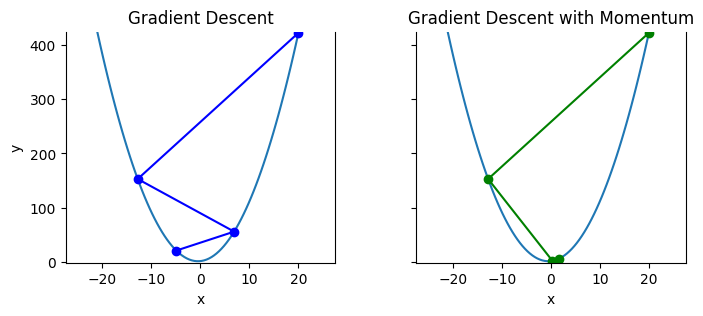
\includegraphics[width=0.5\textwidth]{report/figures/GD_momentum.png}\\
The figure illustrates, on the left, how conventional gradient descent converges towards the minimum of the depicted quadratic function. On the right, one can observe gradient descent enhanced with momentum. Although the initial step is similar for both methods, the subsequent steps differ markedly. In the case of gradient descent alone, only the current gradient is considered as the slope. However, when employing gradient descent with momentum, the direction for the next step is determined by an accumulation of the current gradient and the previous gradients, resulting in a steeper descent as the first gradient slopes upwards.\\
In ADAM the learning rate is manipulated via the first moment estimate vector. The biased form is defined as 
$$m_t=m_{t-1}\cdot \beta_1 + g_t\cdot (1-\beta_1)$$
This is called the biased mean of the gradient at iteration $t$, where $\beta_1$ has the default value of $0.9$. The unbiased mean gradient, defined as $\hat{m_t}$ is then multiplied with the adaptive learning rate and subtracted from $\theta_{t-1}$ to form the adapted set of parameters $\theta$. This inherits ADAM with the properties from Gradient Descent with Momentum as described.\\
It is important to notice that $m_t$ is initialized at $t=0$, being $m_0$, as a vector of zeros. This causes a bias towards $0$, which will be discussed in section \textit{Bias Correction}.


\subsection{Second Moment Vector - Adaptive Learning Rate}
The adaptive learning rate in ADAM adjusts the learning rate by considering the past gradients. This allows the model to take larger steps when far from the minimum and smaller steps when closer. This is possible, as the squared gradient is considered, meaning when the loss (error in a neural network) is large the learning rate is higher, and vice versa. Furthermore, by adjusting the learning rate this way, the initial learning rate is less relevant as it gets adjusted toward the data automatically. The methods idea was first copied from the Adadelta and RMSprop optimizer.
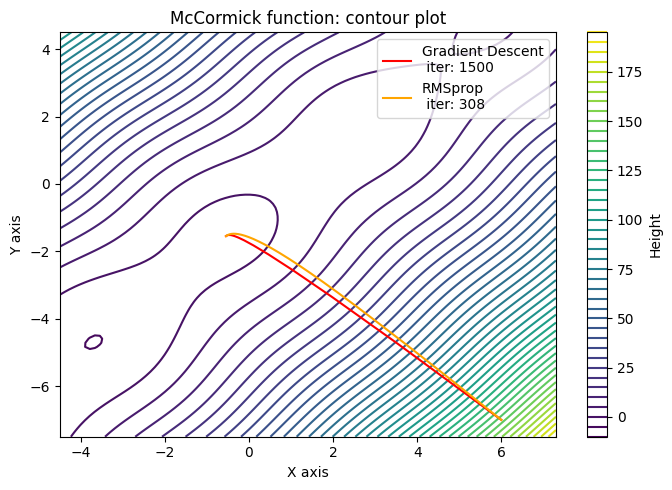
\includegraphics[width=0.5\textwidth]{report/figures/GD_rmsprop.png}\\
The figure shows a contour plot of the McCormick function, regularly explored for optimization due to its landscape. The graph illustrates the difference between classic GD compared to GD with the adaptive learning rate as implemented by ADAM. This is achieved by dividing GD Learning rate by the root of the second moment vector. While classic GD is overshooting during the first couple of steps, GD with adaptive learning takes smaller steps when getting closer to the minimum, as the initial point is already close which adaptive learning knows due to its dependency of the gradient.\\
In ADAM the learning rate is manipulated via the second moment vector. The biased form is defined as:
$$v_t = v_{t-1} \cdot \beta_2 + g_t^2 \cdot (1-\beta_2)$$
This is called the biased uncentered variance of the gradient at iteration $t$. Where $\beta_2$ has a default value of 0.999. The vector $v_t$ is initialized as $v_0$ being a vector of zero causing a bias, similar to $m_t$ that will also be explained in section \textit{Bias Correction}. The squared unbiased second-moment vector $\sqrt{\hat{v_t}}$ divides the default learning rate in ADAM to make it adaptive.\\
%WORKS BETTER FOR HIGH DEMSIONs, to navigate don't get stuck in the local maxima
% write briefly about that
\subsection{Initial Bias Correction}
Bias correction is an essential step to ensure the accuracy and efficiency of the moment vectors, especially during the initial iterations. As both vectors are initialized as vectors of zero a significant bias towards zero is evident in the initial steps. This can lead to smaller-than-ideal step sizes at the start of optimization. If not corrected, this can slow down the convergence of the algorithm, as the optimizer takes conservatively small steps when the step sizes are unduly influenced by the initial bias.\\
Bias correction is performed for both the first and second-moment vector :
\begin{enumerate}
    \item First Moment Bias Correction:\\
    \(m_t\) is corrected by dividing it by \((1 - \beta_1^t)\), where \(\beta_1\) is the exponential decay rate for the first moment estimates, and \(t\) is the iteration step. As \(t\) increases, \((1 - \beta_1^t)\) approaches 1, and the bias correction becomes less significant.
    \item Second Moment Bias Correction:\\
    Similarly, the second-moment vector \(v_t\) is corrected by dividing it by \((1 - \beta_2^t)\), where \(\beta_2\) is the exponential decay rate for the second-moment estimates. This adjustment compensates for the underestimation of the second moment, ensuring that the scaled gradient is divided by a more accurate estimate of its variance, leading to more appropriate step sizes.
\end{enumerate}

% GRAOH FOR INTIAL BIAS CORRECTION
\subsection{Principes performance compared to GD}
% find a nice graph to show how adam
% services local minima compared to gradient descent
\section{The Algorithm}
Definitions as in the forgoing section.
\subsection{Initialize Hyperparameters}
First, the hyperparameters need to be initialized:
\begin{itemize}
    \item $\alpha$ stepsize or the initial learning rate, usually around $0.001$ is picked. As mentioned the learning rate is manipulated by the second moment vector, resulting that the initial hyperparameter $\alpha$ having less impact on the Opimitizer. In general a higher learning rate can lead to faster convergence but risks overshooting the minimum, potentially causing instability. A lower learning rate ensures more stable convergence but may slow down the optimization process, possibly leading to getting stuck in local minima. 
    \item $\beta_1$ is the exponential decay rate for the first moment vector, usually around $0.9$. A higher \(\beta_1\) value (close to 1) gives more weight to past gradients, potentially smoothing out the optimization but risking a slower reaction to recent changes. A lower \(\beta_1\) decreases memory, making it more responsive to new gradients but possibly more volatile.
    \item $\beta_2$ is the exponential decay rate for the second moment vector, usually around $0.999$. A higher \(\beta_2\) value increases the influence of past squared gradients, leading to more stable but smaller learning rates and therefore slower updates, as it might not react quickly to changes in gradient variance. A lower \(\beta_2\) makes the algorithm more sensitive to recent changes in gradient variance, which can accelerate learning but increase the risk of instability.
    \item $\epsilon$ is for computational purposes to avoid division by zero. Can be picked according to computational capabilities between $10^{-5}$ and $10^{-8}$.
\end{itemize}
\subsection{Initialize Model Dependent Parameters}
\begin{itemize}
    \item $f(\theta)$ being the Stochastic loss function with parameters $\theta$. In the context of training neural networks, the stochastic objective function refers to the loss or cost function evaluated on a randomly selected subset (mini-batch) of the training data.
    \item $t=1$ initial step in the algorithm
    \item $\theta_0$ initial parameters
    \item $m_0=0$ first moment vector initializes as a vector of zeros
    \item $v_0=0$ second moment vector initializes as a vector of zeros
\end{itemize}
\subsection{Algorithm steps}
As long as the parameters $\theta_t$ are not converging the following loop runs:
\begin{enumerate}
    \item Compute the gradient \(g_t\) with respect to the parameters \(\theta\) at time step \(t\).\\
    $$g_t= \nabla_{\theta} f_t(\theta_{t-1})$$
    \item Update biased first-moment estimate
    $$m_t = \beta_1 \cdot m_{t-1} + (1 - \beta_1) \cdot g_t$$
    \item Update biased second-moment estimate
    $$v_t = \beta_2 \cdot v_{t-1} + (1 - \beta_2) \cdot g_t^2$$
    \item Compute bias-corrected first-moment estimate
    $$\hat{m}_t = \frac{m_t}{1 - \beta_1^t}$$
    \item Compute bias-corrected second-moment estimate: 
    $$\hat{v}_t = \frac{v_t}{1 - \beta_2^t}$$
    \item Update the parameters
    $$\theta_{t+1} = \theta_t - \alpha \cdot \frac{\hat{m}_t}{\sqrt{\hat{v}_t} + \epsilon}$$
    \item Increase $t$ by one
    \item Check if $\theta_t$ converged
\end{enumerate}




%PRATICAL EXAMPLE
\section{Computational Implementation}
Do a classification.  
Get an example with neural network. Use a general architecture. Maybe image classification (3Blue one Brown, video example).
\subsection{Example Impleementation}
Insert Code

% COMPARISON of performance
\section{Performance Comparison}

 
\section{Conclusion}
Ending




% CODE FOR APPENDIX
\onecolumn
\newpage
\pagestyle{fancy}


\section{Appendix A}
\centering Source Code
All Notebooks and Visualizations including detailed code can be found in our GITHUB Repository with the link: \href{https://github.com/jakthehut/ADAM-Optimizer}{https://github.com/jakthehut/ADAM-Optimizer}


\end{document}